\documentclass[12pt]{article}
\usepackage[left=2cm, top=2cm, right=2cm, bottom=2cm]{geometry}
\usepackage[utf8]{inputenc}
\usepackage[T1]{fontenc}
\usepackage[french]{babel}
\usepackage{graphicx}
\usepackage{graphics}
\usepackage{amsmath}
\usepackage{tikz}
\usepackage{graphicx}
\usepackage{xcolor}
\usepackage{parskip}
\usepackage{physics}


\title{\textbf{Méthodes expérimentales} \\ TP 3: Chaleur spécifique, calorimétrie}
\author{MENARD Alexandre \\ VIEILLEDENT Florent}

\setlength{\parindent}{1cm}

\begin{document}
\maketitle

\section*{Introduction}
Dans ce travail pratique, on déterminera les coefficients thermiques, ainsi que les coefficients thermiques
massiques et molaires de l'eau, du vase et de plusieurs métaux. On évaluera également les fuites thermiques du calorimètre pour mettre
en avant de potentielles erreurs dans nos expériences précédentes. \\
On s'appuiera sur des modèles théoriques pour comparer nos mesures à la théorie. Pour effectuer nos comparaisons, on utilisera
les outils numériques adéquats.


\newpage

\section{Première expérience : Détermination de la capacité thermique de l'eau et du vase calorimétrique}

Le but de cette expérience est de déterminer la capacité thermique de l'eau. On utilisera principalement un calorimètre et une résistance chauffante de $5 \Omega$, 
pour pouvoir établir une relation entre la température de l'eau et le temps passé à chauffer de l'eau. 
On pourra en même temps estimer la capacité thermique du vase calorimétrique. 

\subsection{Expérimentation}

Nous effectuerons la même expérience pour différentes masses d'eau et pour différents voltages. Pour la première série de mesure, on utilise $450g$ d'eau et une tension de $12V$. On remplit la cuve interne du calorimètre avec la masse d'eau souhaitée, qu'on a pesé avec une balance. On agite l'eau pour que cela soit homogène et on relève la température grâce au thermomètre. On met ensuite en place la résistance chauffante dans l'eau. La résistance est branchée à l'alimentation qui est elle même réglée sur $12V$. On lance le chronomètre et on relève la température toutes les minutes et ceci pendant 15 minutes. On mélange l'eau pendant 15 secondes avant la mesure pour s'assurer que la température soit homogène. 

On recommence ensuite l'expérience avec la même masse d'eau mais une tension de $6V$. Pour la dernière série de mesure, on utilise une tension de $12V$ et une masse d'eau de $800g$.

\subsection{Données}

L'incertitude sur la température nous est donnée par le thermomètre et est de $\delta T = 0.2^\circ C$ (valeur issue du manuel du thermomètre trouvé sur le site du constructeur). 
L'incertitude sur la masse est de $\delta m = 0.1g$ (donnée fournie par la balance). 
On estime l'incertitude sur le temps à $\pm 1s$, car c'est le temps que nous mettons pour lire le chronomètre puis le thermomètre. 
L'incertitude sur la tension nous est donnée par la dernière décimale affichée par le générateur, donc $\delta U = \pm 0.1V$.

	Données pour la première expérience, avec $m_{eau1}=450.0\pm 0.1g$ et $U_1=12.0\pm 0.1V$ :


	Données pour la deuxième expérience, avec $m_{eau2}=450.0\pm 0.1g$ et $U_2=6.0\pm 0.1V$ :
	
	
	Données pour la troisième expérience, avec $m_{eau3}=800.0\pm 0.1g$ et $U_3=12.0\pm 0.1V$ :

\newpage
\subsection{Exploitation des données}

On trace le graphique de la température en fonction de la température:

\begin{figure}[h!]
	\begin{center}
		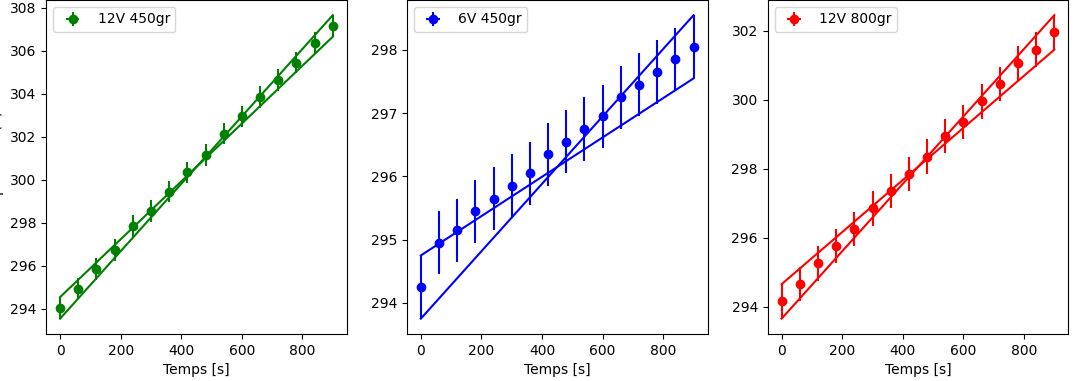
\includegraphics[scale=0.64]{img/Figure_1.png}
	\end{center}
	\label{fig:graph1}
	\caption{Température (en Kelvin) en fonction du temps pour les 3 expériences}
\end{figure}

% Ici, on répond à "Comment évolue la température ? Que cela signifie-t-il ?"
On remarque que la température évolue linéairement, ainsi, la température est fonction du temps, et qu'il existe un coefficient directeur que l'on peut déterminer à l'aide de la méthode des pentes extrêmes.
Dans le cas de la deuxième expérience, on remarque que la température augmente moins rapidement que les deux autres expériences. 

Soient $t_i, t_f, T_i, T_f$, respectivement le temps initial, final et la température initiale et finale. On applique la formule suivante afin d'obtenir le coefficient directeur $a$ ainsi que l'incertitude associée $\delta a$:

\begin{gather*}
	a_{max} = \frac{(T_f + \delta T) - (T_i - \delta T)}{(t_f - \delta t) - (t_i + dt)} \\
	a_{min} = \frac{(T_f - \delta T) - (T_i + \delta T)}{(t_f + \delta t) - (t_i - dt)} \\
	\\
	a = \frac{a_{max} + a_{min}}{2} \\
	\delta a = \frac{a_{max} - a_{min}}{2}
\end{gather*}

On obtient donc les valeurs suivantes grâce à cette méthode pour les trois expériences:
\begin{itemize}
	\item Expérience 1: $a_1 = 0.0146 K.s^{-1}$ et $\delta a_1 = 0.0005 K.s^{-1}$
	\item Expérience 2: $a_2 = 0.0042 K.s^{-1}$ et $\delta a_2 = 0.0005 K.s^{-1}$
	\item Expérience 3: $a_2 = 0.0087 K.s^{-1}$ et $\delta a_3 = 0.0005 K.s^{-1}$
\end{itemize}

De façon plus générale, on posera $\delta a = 0.0005 K.s^{-1}$ pour les trois expériences.

\newpage
\subsubsection{Calcul théorique, résultat attendu}

Dans notre système, on trouve deux parties, l'eau de masse $m_{eau}$ et le vase de masse $m_{vase}$ en aluminium. Ainsi, la capacité thermique totale (grandeur extensive) de notre système est donc:

\begin{equation}
	C_V = m_{eau}c_{eau}+ m_{vase} c_{vase}
\end{equation}

En posant que $c_{eau} = 4185 J.kg^{-1}.K^{-1}$ et $c_{vase} = 921 J.kg^{-1}.K^{-1}$ (car constitué d'aluminium), on peut déterminer la valeur théorique de $C_V$ que l'on doit obtenir par l'expérience:

\begin{table}[h!]
	\begin{center}
		\begin{tabular}{|c|c|c|c|c|}
			\hline
			Expérience n° & $m_{eau}$ (en kg) & $m_{vase}$ (en kg) & $C_V$ (en $J.K^{-1}$) & $C_V(eau)$ (en $J.K^{-1}$)\\ \hline
			1 & 0.450 & 0.0969 & $1973$ & $1883$ \\
			2 & 0.450 & 0.0969 & $1973$ & $1883$ \\
			3 & 0.800 & 0.0969 & $3437$ & $3348$ \\ \hline
		\end{tabular}
	\end{center}
	\caption{Calcul théorique de la capacité thermique totale}
\end{table}

Si le vase est négligeable, on doit trouver une valeur aux alentours de $1883$ $J.kg^{-1}.K^{-1}$ ou $3348$ $J.kg^{-1}.K^{-1}$ selon l'expérience. Si l'on trouve un résultat différent, 
on pourra en déduire que la capacité du vase n'est pas négligeable.

\subsubsection{Calcul expérimental, résultat obtenu}
Le système \{eau+vase calorimétrique\} est liquide pour l'eau, et solide pour le vase.
Ainsi, le volume est constant et la pression aussi. La relation pour la chaleur est donc:

\begin{equation}
\delta Q=C_VdT
\end{equation}

avec $\delta Q$ la chaleur fournie et $C_V$ la capacité thermique. 

On suppose que $C_V$ est constant sur la gamme de température utilisée, on a donc:

\begin{equation}
Q = C_V\Delta T = P\Delta t
\end{equation}

avec P la puissance fournie et $\Delta t$ la durée pendant laquelle on a injecté du courant dans la résistance.

On néglige dans un premier temps la présence du vase calorimétrique, de cette façon, nos mesures devraient fournir directement la valeur de $C_{eau}^{exp}$, la capacité thermique de l'eau.
En déterminant la valeur de $C_{eau}^{exp}$ pour chaque expérience, on pourra les comparer à la valeur théorique $C_V$ déterminer plus tôt et déduire si l'on peut réellement négliger le vase ou non.

\begin{equation}
	C_{eau}^{exp} \Delta T = U I \Delta t \Rightarrow C_{eau}^{exp} = \frac{U I \Delta t}{\Delta T} = \frac{U^2\Delta t}{R \Delta T}
\end{equation}

\newpage
Pour calculer notre incertitude, on utilise la méthode des dérivées partielles:

\begin{align*}
	\delta C_{eau}^{exp} & = \abs{\frac{\partial C_{eau}^{exp}}{\partial U}} \delta U + \abs{\frac{\partial C_{eau}^{exp}}{\partial \Delta T}} \delta (\Delta T) + \abs{\frac{\partial C_{eau}^{exp}}{\partial \Delta t}} \delta (\Delta t)\\
	& = \frac{2U \Delta t}{R \Delta T} \delta U + \frac{U^2 \Delta t}{R \Delta T ^2} \delta (\Delta T) + \frac{U^2}{R \Delta T} \delta (\Delta t)\\
\end{align*}

On obtient les résultats suivants pour les 3 expériences:
\begin{table}[h!]
	\begin{center}
		\begin{tabular}{|c|c|c|c|c|}
			\hline
			Expérience n° & $C_{eau}^{exp}$ (en $J.K^{-1}$) \\ \hline
			1 & $1978 \pm 111$ \\
			2 & $1705 \pm 283$ \\
			3 & $3323 \pm 272$ \\ \hline
		\end{tabular}
	\end{center}
	\caption{Valeur de $C_{eau}^{exp}$ pour les 3 expériences}
\end{table}

Nos incertitudes sont bien trop grandes pour pouvoir conclure sur la négligeabilité du vase dans notre système.
Cependant, on peut tout de même utiliser ces valeurs lorsque l'on a besoin de la capacité thermique du système entier.

On doit donc utiliser une approche différente afin de distinguer la capacité thermique du vase et celle de l'eau. On note désormais $C_V = C_{eau}^{exp}$, car dans nos valeurs de $C_{eau}^{exp}$, 
on a les deux capacités thermiques. On distingue les capacités thermiques de chaque expérience en notant $C_{V1}, C_{V2}, C_{V3}$. On a donc le système suivant:

\begin{align*}
	\begin{cases}
		C_{V1}=C_{eau1}+C_{vase} \\
		C_{V3}=C_{eau3}+C_{vase}
	\end{cases} 
&\Rightarrow 
	\begin{cases}
		C_{vase}= C_{V1} - m_{eau1} \times \frac{C_{V3}-C_{V1}}{m_{eau3} - m_{eau1}} \\
		c_{eau} = \frac{C_{V3}-C_{V1}}{m_{eau3} - m_{eau1}}
	\end{cases}
\end{align*}

On peut enfin faire l'application numérique et obtenir $C_{vase}$ et $c_{eau}$:
\begin{align}
	c_{eau} = 3843 \pm 1127 J.kg^{-1}.K^{-1} & \quad C_{vase} = 248 \pm 618 J.K^{-1}
\end{align}


\subsubsection{Conclusion et interprétation}
En théorie, la valeur de $c_{eau}$ est de $4185$ $J.kg^{-1}.K^{-1}$ et la valeur de $c_{vase}$ est $897$ $J.kg^{-1}.K^{-1}$ soit dans notre cas $C_{vase}^{th} = m_{vase} * c_{vase} \approx 87 J.K^{-1}$ et $C_{vase}^{th} = m_{eau} * c_{eau} \approx 87 J.K^{-1}$
Nos mesures permettent de voir que $c_{eau}$ ainsi que $C_{vase}$ avec des incertitudes sont dans les valeurs théoriques, cependant, nos incertitudes représentent environ 25\% pour $c_{eau}$
et 300\% pour $C_{vase}$ ce qui rend nos résultats inutilisables pour interpréter une quelconque valeur de $c_{eau}$ ou $C_{vase}$. 

Nous avons exploré la possibilité d'erreur dans nos calculs d'incertitudes et d'erreurs de calculs. Il reste la possibilité que nos mesures soient erronées, que nos appareils de mesures soient également pas suffisament précis 
pour atteindre une précision satisfaisante pour détecter un écart de la capacité thermique à celle théorique. En conclusion, il serait nécessaire de reproduire cette expérience afin de voir si l'on retrouve les mêmes résultats afin de déterminer le type d'erreurs que nous avons rencontré.

\newpage
\section{Deuxième expérience : Capacités thermiques massiques de quelques solides}

Le but de cette expérience est de déterminer la capacité massique du duralumin, du laiton, du téflon et du plexiglas. On utilisera pour cela la relation suivante:

\begin{equation}
	T_f=\frac{C_0T_0+C_1T_1}{C_0+C_1}
\label{EquationTf}
\end{equation}
avec $C_0$ la capacité thermique du système \{eau+vase\}, $C_1$ la capacité thermique du métal, $T_0$ la température initiale de l'eau, $T_1$ la température initiale du métal et $T_F$ la température finale de l'eau.

\subsection{Expérimentation}

On place $450g$ d'eau dans le calorimètre et on mesure sa température après avoir agité. On place un morceau du solide qu'on souhaite étudier dans de l'eau bouillante, dont on mesure aussi la température. 
Après quelques minutes, on retire le solide de l'eau bouillante et on le met dans le calorimètre. 
On agite en continu l'eau tout en surveillant la température. On note cette dernière lorsqu'elle atteint un maximum. 
On retire ensuite le solide et on le pèse après l'avoir séché.

\subsection{Données}
On reprend les notations de l'équation (\ref{EquationTf}). Les incertitudes sont données par la balance et le thermomètre. Pour tous les solides, on a $T_1=94.6\pm 0.2^{\circ}C$ (issu du manuel du thermomètre):
\begin{table}[h!]
	\begin{center}
		\begin{tabular}{|c|c|c|c|c|}
		\hline
		Solide & $m_{eau} \pm 0.1g$ & $m_{solide}\pm 0.1g$ & $T_0\pm 0.2^{\circ}C$ & $T_f\pm 0.2^{\circ}C$\\ \hline
		Laiton & $451.1$ & $82.7$ & $21.1$ & $22.4$ \\
		Téflon & $451.1$ & $32.5$ & $22.3$ & $23.4$ \\
		Plexiglas & $450.0$ & $47.8$ & $22.3$ & $23.4$ \\
		Duralumin & $452.5$ & $77.2$ & $21.1$ & $24.0$ \\ \hline
		\end{tabular}
		\caption{Mesures pour les différents solides de l'expérience 2}
		\label{table:mesureexp2}
	\end{center}
\end{table}

\subsection{Exploitation des données}
On détermine la capacité thermique $C_0$ du système en utilisant les valeurs théoriques des capacités thermiques $c_{eau}=4185\, J.kg^{-1}.K^{-1}$ et $c_{aluminium}=897 J.kg^{-1}.K^{-1}$. On a mesuré $m_{vase}=96.9\pm 0.1g$
\begin{equation}
C_0=c_{eau}m_{eau}+c_{aluminium}m_{vase}
\end{equation}

Calcul des incertitudes:
\begin{align*}
\delta C_0&= \abs{\frac{\partial C_0}{\partial m_{eau}}} \delta m_{eau} + \abs{\frac{\partial C_0}{\partial m_{vase}}} \delta m_{vase}\\
&=c_{eau}\delta m_{eau}+c_{aluminium}\delta m_{vase}
\end{align*}

On cherche la capacité thermique molaire des matériaux. On va déterminer la capacité thermique du solide grâce à l'équation (\ref{EquationTf}):
\begin{align*}
T_f=\frac{C_0T_0+C_1T_1}{C_0+C_1} &\Rightarrow T_FC_0+T_FC_1=C_OT_0+C_1T_1 \\
&\Rightarrow C_1(T_F-T_1)=C_0(T_0-T_F) \\
&\Rightarrow C_1=\frac{C_0(T_0-T_F)}{T_F-T_1}
\end{align*}

On calcule l'incertitude associée:
\begin{align*}
\Delta C_1 &= \abs{\frac{\partial C_1}{\partial C_0}} \Delta C_0 + \abs{\frac{\partial C_1}{\partial T_0}} \Delta T_0 + \abs{\frac{\partial C_1}{\partial T_1}} \Delta T_1 + \abs{\frac{\partial C_1}{\partial T_F}} \Delta T_F \\
&= \frac{T_0-T_F}{T_F-T_1}\Delta C_0 + \frac{C_0}{T_1-T_F} \Delta T_0 + \frac{C_0(T_F - T_0)}{(T_F-T_1)^2}\Delta T_1 + \frac{C_0(T_F - T_0)}{(T_F-T_1)^2}\Delta T_F
\end{align*}

On peut calculer la capacité thermique massique pour chaque solide:
\begin{equation}
c_{solide}=\frac{C_1}{m_{solide}}
\end{equation}
\begin{align*}
\delta c_{solide}&=\abs{\frac{\partial c_{solide}}{\partial C_1}}\delta C_1 + \abs{\frac{\partial c_{solide}}{m_{solide}}}\delta m_{solide} \\
&=\frac{\delta C_1}{m_{solide}}+ \frac{C_1}{(m_{solide})^2}\delta m_{solide}
\end{align*}


Pour chaque métal, on obtient les valeurs suivantes pour les capacités thermiques et les capacités thermiques massiques avec les incertitudes associées:

\begin{table}[h!]
	\begin{center}
		\begin{tabular}{|c|c|c|}
			\hline
			Métal & $C_{solide}$ (en $J.K^{-1}$) & $c_{solide}$ (en $J.kg^{-1}.K^{-1}$)\\ \hline
			Laiton & $36 \pm 11$ & $430 \pm 135$ \\
			Téflon & $31 \pm 11$ & $939 \pm 350$ \\
			Plexiglas & $30 \pm 11$ & $637 \pm 237$ \\
			Duralumin & $67 \pm 12$ & $872 \pm 152$ \\ \hline
		\end{tabular}
	\end{center}
	\caption{Valeur des capacités thermiques pour les différents solides de l'expérience}
\end{table}

Il faut maintenant calculer la masse molaire de chaque matériau. On a déjà la formule brute du plexiglas ($C_5H_8O_2$) et du téflon ($C_2F_4$). On a les masses molaires suivantes:
\begin{align*}
M_{plexiglas}&=5M_C+8M_H+2M_O & M_{teflon}&=2M_C+4M_F  \\
&=5\times 12+8+2\times 16 & &=2\times 12+4\times 19 \\
&=100\, g.mol^{-1} & &=100\, g.mol^{-1}
\end{align*}

Pour le laiton et le duralumin, il faut calculer la masse molaire du matériau à partir des proportions massique qu'on note $w_{i}$. On a :
\begin{align*}
M_{solide}&=\frac{m_{totale}}{n_{totale}} & w_i=\frac{m_i}{m_{totale}}
\end{align*} 

Pour un alliage de métaux, on a :
\begin{align*}
n_{totale}&=\sum_{i}n_i
=\sum_i \frac{m_i}{M_i}
=\sum_i \frac{m_{totale}w_i}{M_i}
\end{align*}

On injecte dans la précédente équation et on obtient:
\begin{equation}
M_{solide}=\frac{1}{\sum_{i} \frac{w_i}{M_i}}
\end{equation}

On fait l'application numérique pour le laiton et le duralumin avec:

\begin{itemize}
	\item les fraction massiques pour le laiton: $w_{zinc}=0.4$, $w_{plomb}=0.02$, $w_{cuivre}=0.58$
	\item les fractions massiques pour le duralumin: $w_{silicium}=0.005$, $w_{fer}=0.0035$, $w_{cuivre}=0.04$, $w_{manganese}=0.007$, $w_{magnesium}=0.007$, $w_{zinc}=0.0025$, $w_{aluminium}=0.935$
\end{itemize}

On obtient:
\begin{align*}
M_{laiton}&=65.2\, g.mol^{-1} & M_{duralumin}&=27.8\, g.mol^{-1}
\end{align*}
 
On utilise maintenant les relations $c_{molaire}=c_{solide}M_{solide}$ et $\delta c_{molaire}=c_{solide}\delta M_{solide} + M_{solide}\delta c_{solide }$ puis on regroupe nos résultats dans un tableau.
\begin{table}[h!]
	\begin{center}
		\begin{tabular}{|c|c|c|c|c|}
		\hline
		Solide & $C_0\pm 0.5(J.K^{-1})$ & $C_1(J.K^{-1})$ & $c_{solide}(J.kg^{-1}.K^{-1})$ & $c_{molaire}(J.mol^{-1}.K^{-1})$ \\
		\hline
Laiton    & $1977.1$ & $36 \pm 11$ & $430 \pm 135$  & $28 \pm 9$ \\
Téflon    & $1977.1$ & $31 \pm 11$ & $939 \pm 350$  & $94 \pm 35$ \\
Plexiglas & $1972.5$ & $30 \pm 11$ & $637 \pm 237$  & $64 \pm 24$ \\
Duralumin & $1983.0$ & $67 \pm 12$ & $872 \pm 152$ & $24 \pm 4$ \\
		\hline	 
		\end{tabular}
	\end{center}		
\end{table}

\subsection{Conclusion}
Dans cette expérience, on a réussir à obtenir des résultats satisfaisant avec des capacités thermiques massiques proches des valeurs théoriques. Cependant, on notera un seul solide qui 
n'a pas une capacité thermique massique correspondante à celle théorique. Selon nos mesures, on déduit que $c_{plexiglas} \in [400, 874]$, ce qui est environ la moitié de la valeur théorique avec $c_{plexiglas}^{th} \approx 1400 J.kg^{-1}.K^{-1}$.

L'erreur viendrai de la manière dont nous avons réalisé l'expérience. De part la grande valeur de la capacité thermique massique du plexiglas, il faut presque 2 fois plus d'énergie pour élever d'un degré le plexiglas
par rapport aux autres solides à masse égale. Or, nous avons laissé pendant le même laps de temps les solides dans l'eau bouillante. Le plexiglas n'a donc peut-être pas eu le temps suffisant pour s'élever à la température de l'eau bouillante.
Bien que l'extérieur était bien à $94^\circ C$ en ayant mesuré avec le thermomètre, il nous était impossible de s'assurer que le centre ait atteint une telle température. Ainsi, reproduire l'expérience serait important pour effectuer de nouveau la mesure
en laissant plus longtemps le plexiglas afin de s'assurer que le centre soit à température.



\section{Troisième expérience : Évaluation des fuites thermiques du calorimètre}
Le but de cette expérience est d'évaluer les fuites thermiques du calorimètre. On va pour cela reproduire les paramètres d'expérimentations de la première expérience mais sans faire chauffer l'eau (sans brancher la résistance).
\subsection{Expérimentation}

Pour réaliser notre série de mesure, on conserve la même configuration que les expériences précédentes, c'est-à-dire
que l'on conserve la résistance, l'agitateur et le thermomètre pour ne pas fausser nos valeurs. 

On place dans dans le vase du calorimètre 400gr d'eau à $40^\circ C$. On mesure ensuite la température de l'eau à $40^\circ C$ et on mesure la température du calorimètre toutes les 2 minutes pendant 20 minutes.
Afin de simplifier la lecture et la visualisation de la température, on préfère remplacer le tableau par le graphique suivant:

\begin{figure}[h!]
	\begin{center}
		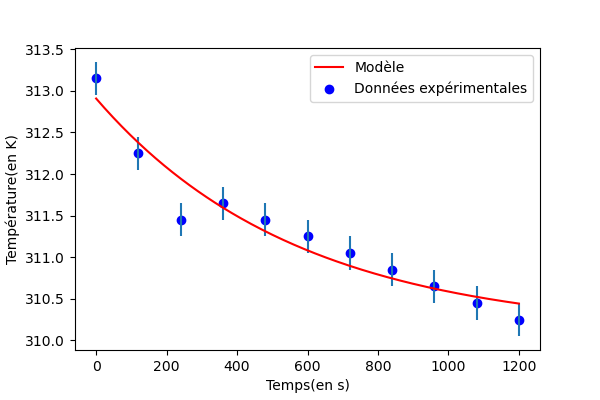
\includegraphics[scale=0.64]{img/Figure_2.png}
	\end{center}
	\label{fig:graph2}
	\caption{Température (en degré celsius) en fonction du temps modélisant la perte de chaleur du calorimètre.}
\end{figure}

\newpage
\subsection{Comparaison de nos résultats avec le modèle théorique}
Le modèle théorique prévoit une décroissance exponentielle de la température du calorimètre avec:

\begin{equation}
	T_{int} = T_{ext} + (T_{int, 0} - T_{ext}) e^{- \frac{t}{R_{th}C}}
\end{equation}

avec les grandeurs suivantes:
\begin{itemize}
	\item $T_{int}$ : température interne du calorimètre
	\item $T_{ext}$ : température extérieur
	\item $T_{int, 0}$ : température interne du calorimètre à l'instant initial
	\item $C$: capacité thermique du calorimètre
\end{itemize}

Ainsi, on peut exprimer le logarithme de cette courbe pour obtenir une droite:

\begin{align*}
	T_{int} - T_{ext} = (T_{int, 0} - T_{ext}) e^{- \frac{t}{R_{th}C}} & \Rightarrow \ln(T_{int} - T_{ext}) = \ln(T_{int, 0} - T_{ext}) - \frac{t}{R_{th}C} \\
\end{align*}

On trouve donc une expression de droite de la forme:

\begin{equation}
	y = at + b, \text{ avec } a = - \frac{1}{R_{th}C}, b = \ln(T_{int, 0} - T_{ext})
\end{equation}

Pour vérifier que nos mesures correspondent donc à une décroissance exponentielle, on trace cette même courbe en prenant le logarithme. On obtient donc:

\subsection{Conclusion et interprétation}
On a montré que le flux de chaleur n'était pas négligeable. Cette perte d'énergie se traduit donc par des erreurs dans les mesures réalisées, car une partie de la chaleur s'échappe et fait donc baisser la température qu'on lit
avec le thermomètre. Dans la première expérience, nous avons considéré l'enceinte comme adiabatique, ainsi, il n'y a aucune perte de chaleur, on avait donc:

\begin{equation}
	Q = C_V \Delta T
\end{equation}

Or, on perd de la chaleur car l'enceinte n'est pas parfaitement adiabatique. En posant $Q_{fuite} < 0$, la quantité de chaleur perdue, il vient que:

\begin{equation}
	Q = C_V \Delta T + Q_{fuite}
\end{equation}

On a ensuite que le flux de chaleur (en Watts soit $J/s$) s'exprime comme:

\begin{equation}
	\Phi = - \frac{\Delta T}{R_{th}}
\end{equation}

On peut donc en déduire la quantité de chaleur perdue sur une durée avec:

\begin{equation}
	Q_{fuite} = \Phi \times \Delta t = - \frac{\Delta T}{R_{th}} \times \Delta t
\end{equation}

Finalement, il vient que:

\begin{equation}
	Q = C_V \Delta T - \frac{\Delta T}{R_{th}} \times \Delta t = \Delta T \left( C_V - \frac{\Delta t}{R_{th}} \right)
\end{equation}

\section{Conclusion}

\end{document}
